\documentclass[letterpaper,10pt]{article}

\usepackage{epsfig}
\usepackage{wrapfig,float}

\DeclareGraphicsExtensions{.pdf,.png,.jpg}
\graphicspath{ {./Figures/} }

\begin{document}

\date{}

\title{\Large Pony: An Information Retrieval System \\ \small Indexing, Vector Space Searching, OKAPI BM25 Searching, Web Crawler}


\author{{\rm Giannis Apostolidis}\\
				{\rm japostol@csd.uoc.gr}\\
				\and
				{\rm Michalis Athanasakis}\\
				{\rm michath@csd.uoc.gr}\\
}
\maketitle
\section{Abstract}
Information retrieval systems are continuously gain attention through the last fifteen years after the explosion of the Internet. A good performing search engine is always useful and can introduce new understanding of a dataset. We introduce \emph{ Pony}, a modern offline indexing and search engine for documents.

\section{Introduction}
Our implementation is separated under three basic components.\emph{ Indexing}, \emph{ Searching}, \emph{ Graphics User Interface}(GUI). Each component can provide functionality separated from the rest, except GUI. In the phase of indexing the system is guided to a directory of documents for indexing and performs an indexing algorithm described below to finally store a custom file database to the hard drive. In the phase of searching the program retrieves the database stored from the indexing phase and performs searches using two different algorithms. The program can be executed from a terminal but also provides a GUI functionality to improve usability. Under the GUI mode the user can perform both indexing and searching with just importing the directory of documents to be searched. All parts of the program are implemented with {\tt Java}.

\section{Internals}
For the need of this project we implemented a custom database to store all the necessary information without spending unnecessary size on the disk. The database is separated in three big parts that can be accessed separately from the disk. This enables us to fetch things from the disk when is only necessary during the searching phase. The only part that is on memory while the phase of search is the database of the words(terms) that our system has indexed. The below figures provides an abstract idea on how our system is implemented and how a term is indexed and searched respectively.

\begin{figure}[H]
    \centering
    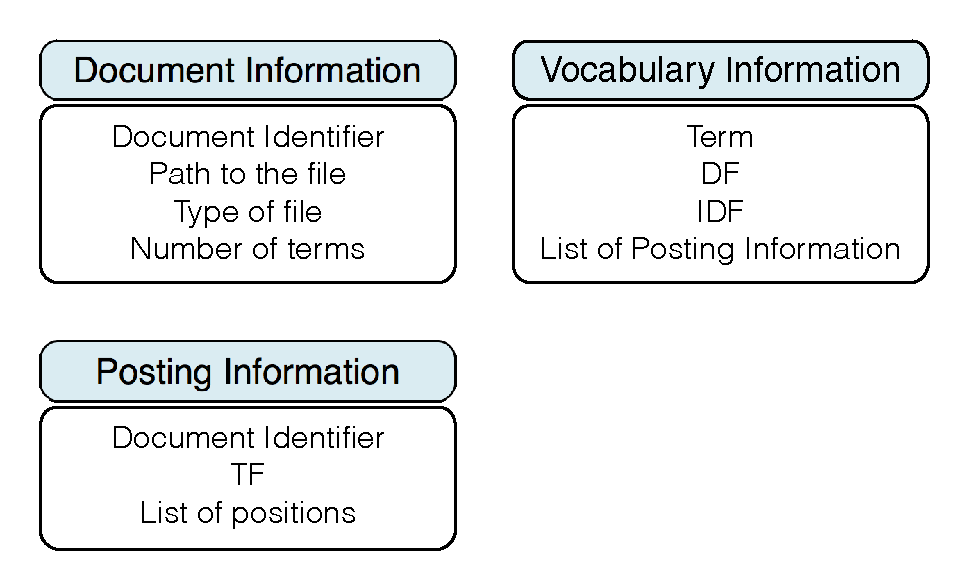
\includegraphics[width=3.2in]{ClassInternals.eps}
    \caption{Structure of information entries}
    \label{Structure of information entries}
\end{figure}

The backbone of the database is the Vocabulary database where all unique terms are indexed and later searched. The Vocabulary database is populated during the indexing phase with with all unique terms located inside the document collection. Inside each Vocabulary Entry(Vocabulary Information in the figure) the system store some information and some pointers to other parts of the database for fast access. For each term there is a list of Posting information which it provides more specific information. Posting information holds the document identifier, calculations and the locations of each sighting of the term inside the specific document. Creating a Posting information list for each term essentially provides the system with information about all the sightings of each term. With the usage of the document identifier we can later retrieve the document information, retrieve the file and complete the search. The final output provides plenty of information about the location and the similarity of the returned document to the specific search we request.

\begin{figure}[H]
    \centering
    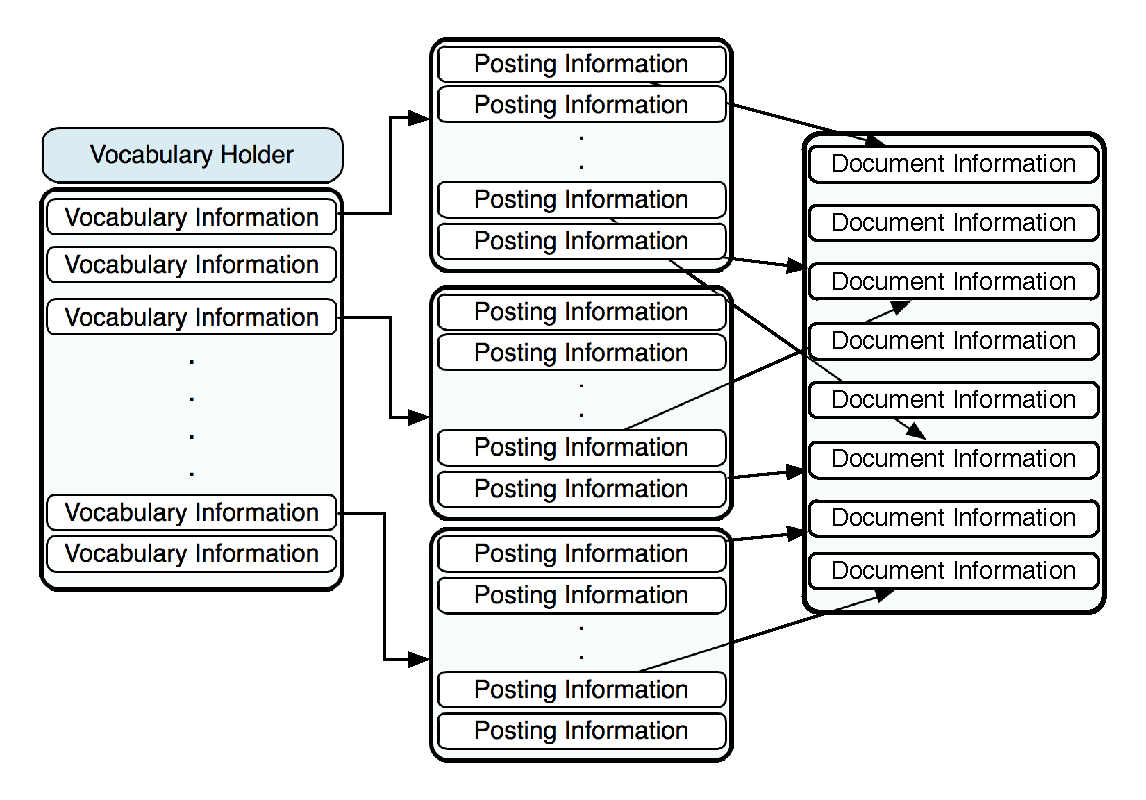
\includegraphics[width=3.2in]{DB.eps}
    \caption{Database structure}
    \label{Database structure}
\end{figure}

When we use the term \emph{ list} we imply a data structure responsible to store the information. The actual implementation for each specific data structure is chosen after considering each special characteristic of that part of the database and other factor, performance on writing and on reading.

\section{Indexing}
The phase of \emph{ Indexing} is the phase where the database is initialized using a specific document collection provided by the user. This phase can be done both by terminal or the GUI our system offer. The system has the ability to index documents type of {\it .txt} with UTF-8 encoding. This provides the ability to index documents in languages different of English. Pony also offer the functionality of stop words, words that when located in the documents are ignored. Along with the stop words specific types of data are ignored. The user has the ability to select a directory with the stop words files of his choice to feed the system to alter the indexing terms. After the valid words have been processed another part of the algorithm is to provide some \emph{ stemming} functionality to improve the indexing. The list below provides the types and the behavior the system has on them.

\begin{description}
  \item[Numbers] All digits are ignored from the search. In the case a digit is located inside a word during indexing then the word is separated into two words, the word before the digit and the word after. After that, each of the newly created word is again processed to finally separate all the words from the numbers. All the terms are then processed into indexing.
  \item[Symbols] A large variety of symbols are ignored during the search. In the case a symbol is located inside a word during indexing then the word is separated into two words, the word before the symbol and the word after. After that, each of the newly created word is again processed to finally separate all the words from the symbols. All the terms are then processed into indexing.

  List of all the symbols can be located inside the directory: 

{\tt /src/PonyIndexer/stopWords.java}
\end{description}

\section{Searching}
Searching is the second phase of this system. After all the documents are indexed the user can search in them. The search returns a bundle of information to help the user understand how similar is the document that was returned regarding his search terms. Along with that snippet of text of the documents are returned along with the specific offset from the start of the file where the term is located. The search engine provides the same functionality with the usage of stop words and by ignoring the same numbers and symbols. Also, the search engine ignores the capital and lower letters improving the returning results. In some languages like Greek also punctuation marks are also ignored to offer another improvement. Finally, the search terms are also being stemmed to offer compatibility between indexing and searching.

The actual searching algorithm has been implemented using two separated models. The one model is the \emph{ Vector Space} Model and the other is based on the \emph{ OKAPI BM25} standard.

\begin{figure*}
    \centering
    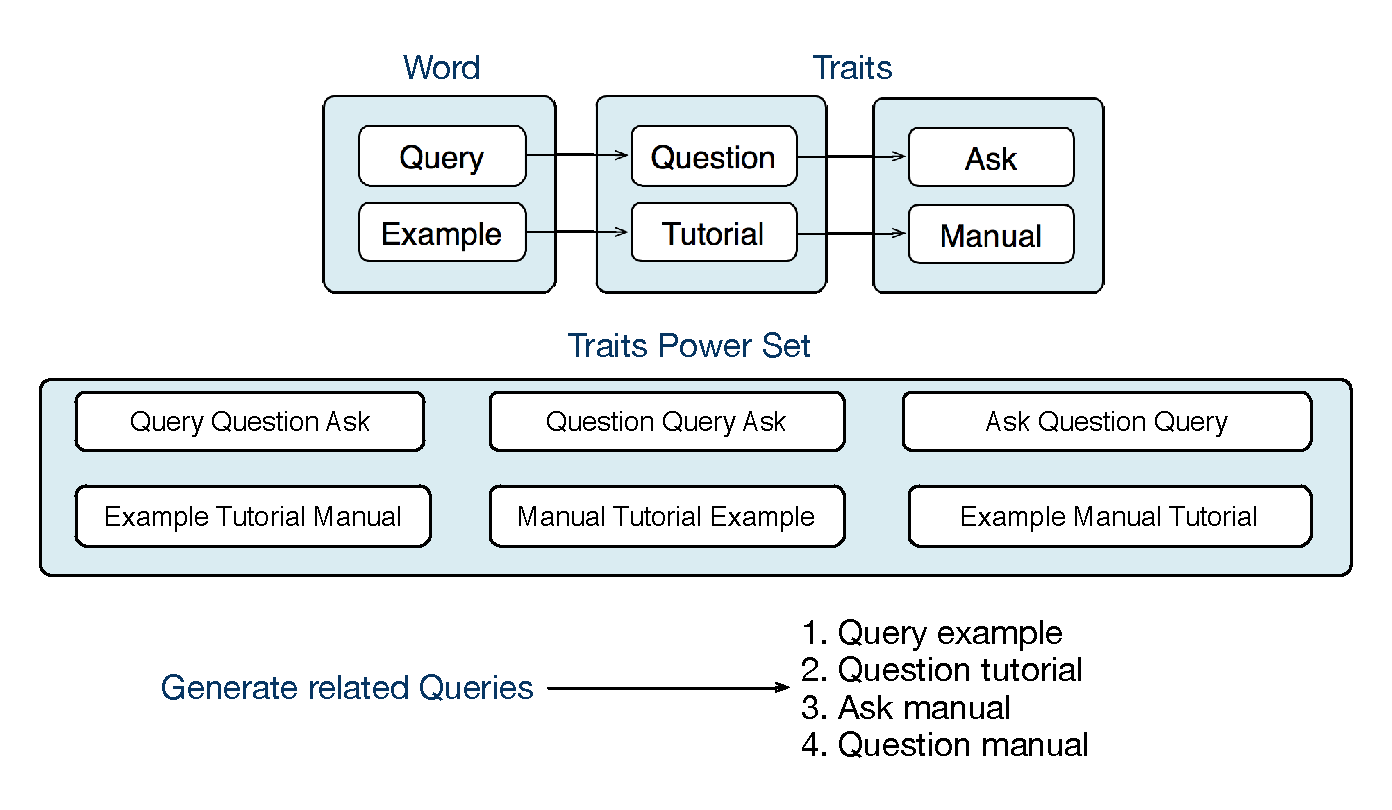
\includegraphics[width=4.0in]{RelatedQuery.eps}
    \caption{Generation of related queries}
    \label{Generation of related queries}
\end{figure*}

\section{Searching Optimizations (\emph{Phase B})}
Searching Optimizations are separated in two different aproaches. Both schemes utilize the \emph{Universal Word net(UWN)} to fetch related words to each term of the query. The first scheme tries to improve accuracy by adding specific terms to the inputed query from the user. For each query term the UWN returns a list of words, their lexicograph family and how related are with the term. Using these data the most related synonyms, hyperonysms, hypnonysms, holonyms and meronyms are selected and inserted into the actual query. This scheme improves the accuracy and the raw findings of the search engine by returning a subset of documents that may not contain the actual terms but their closest related words. The other optimization scheme is the generation of Related Queries to suggest to the user. It is possible a user might not know how to express a question he/she has and the suggestions of related queries can help improve the search by expressing the same or similar questions. The way this scheme works is through a related query component. This component is trying to generate related queries using a list of words and their traits as input. The typical procedure is seperated into two basic steps. First, it calculates a power set using each word's traits. This procedures produces as a result a list of words that has a list of power set of traits. In the second step it is trying to extract the newly generated related queries using the power set as an input. We can assume that a related query is one column from the traits of the powerset list.

\begin{figure}[H]
    \centering
    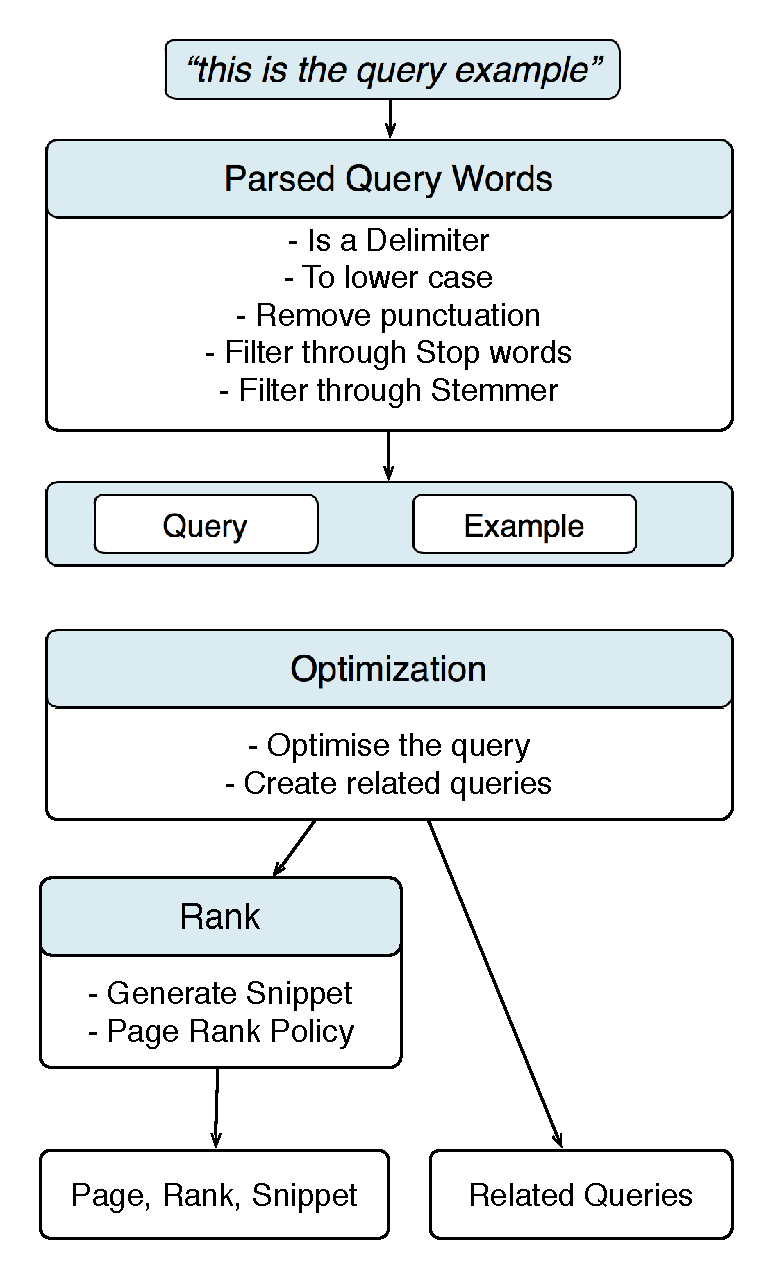
\includegraphics[width=2.5in]{Query.eps}
    \caption{Query structure}
    \label{Query structure}
\end{figure}



\section{GUI}
The system provides command line functionality but the user is advised to prefer the GUI interface for better optical and structured results. The GUI provides functionality to both index and search documents. If a document indexing database does not exist the GUI being provided with the documents collection directory and a stop words directory can index them and "export" a database. If the database already exists in the specified directory the search engine loads it and is ready to provide search functionality. After the search the results are being displayed inside the same GUI along with a variety of information.

\section{Web Crawler}
Web crawler is a mining tool over the web. The purpose of this tool is to download as many web pages as possible to a target storing layer. This tool can be used as the first step of a search engine. The main functionality is the following:
\begin{enumerate}
  \item Download a web page given as argument.
  \item Parse the page using a Xml parser.
  \item Find all the {\tt a} tags, and extract the href attribute.
  \item Save only the text content of the page.
  \item Repeat the same procedure for every extracted href, as many times as the depth argument.
\end{enumerate}

\section{Evaluation}

After the design and the implementation of our system we provide a evaluation
under 3 scopes. The first two scopes are combined under section "Time \& Space
Evaluation". The other section describes the accuracy and what are the expected
results from the system, both in Phase A and Phase B where our optimization are
used.

\subsection{ Time \& Space Optimizations }

In this section there are 8 charts and graphs to provide information on how the
system is being evaluated under many different aspects. What we notice are the
following. 

\begin{itemize} 
\item The size of the indexing files are almost as much size of
the document collection we examine. Still, we believe that when the document
collection will get even bigger the size of indexing database will not change
that drastically.
\item Due to changes in the implementation of Phase B the
searching mechanism is even faster and returns better and more ordered
documents.
\item Even when we run the evaluations multiple times, one hundred times
for each number of query terms times four times the minimum and maximum times
are pretty random and are related to what the rest of the system does that 3
ms. The average values shows how stable the system is.  
\end{itemize}

\begin{figure}[H]
    \centering
    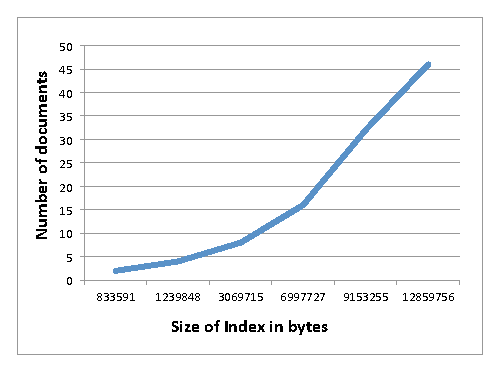
\includegraphics[width=4in]{docNumber-indexSize.eps}
    \caption{ Number of document collection and their respective size of the index database. }
    \label{Query structure}
\end{figure}

\begin{figure}[H]
    \centering
    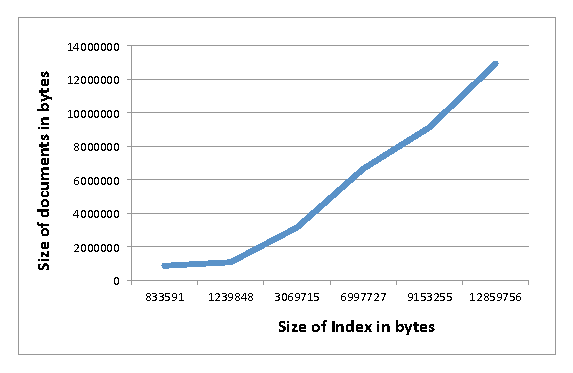
\includegraphics[width=4in]{DocSize-IndexSize.eps}
    \caption{ Size of document collection and their respective size of the index database. }
    \label{Query structure}
\end{figure}

\begin{figure}[H]
    \centering
    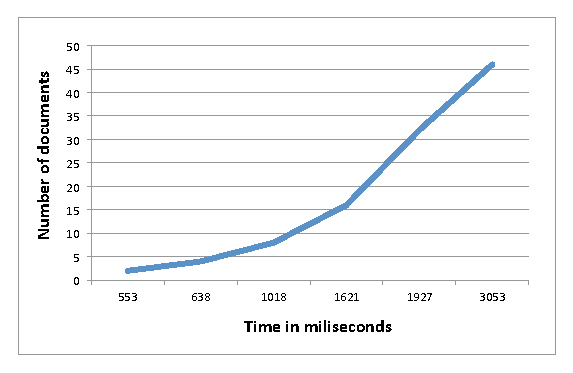
\includegraphics[width=4in]{docNumber-Time.eps}
    \caption{ Size of document collection and the time it is required for indexing. }
    \label{Query structure}
\end{figure}

\begin{figure}[H]
    \centering
    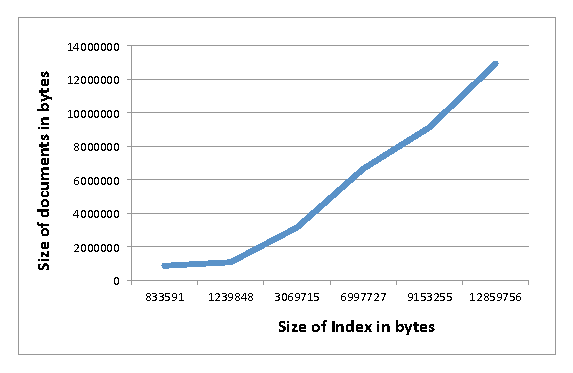
\includegraphics[width=4in]{docSize-Time.eps}
    \caption{ Size of document collection and the time it is required for indexing. }
    \label{Query structure}
\end{figure}

\begin{figure}[H]
    \centering
    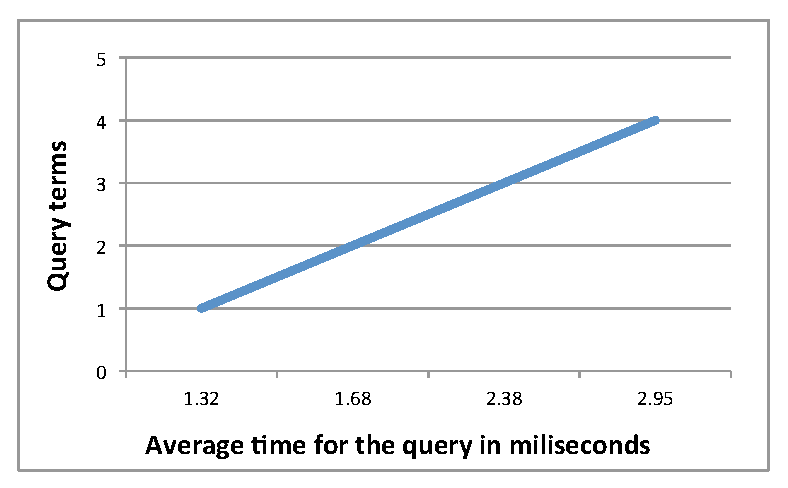
\includegraphics[width=4in]{queryterms-timeA.eps}
    \caption{ Length of the query and average time to search for system A. }
    \label{Query structure}
\end{figure}

\begin{figure}[H]
    \centering
    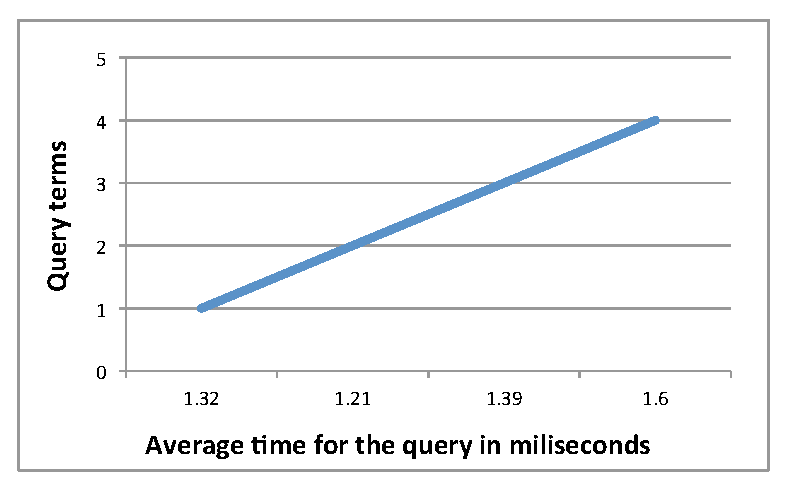
\includegraphics[width=4in]{queryterms-timeB.eps}
    \caption{ Length of the query and average time to search for system B. }
    \label{Query structure}
\end{figure}

\begin{figure}[H]
    \centering
    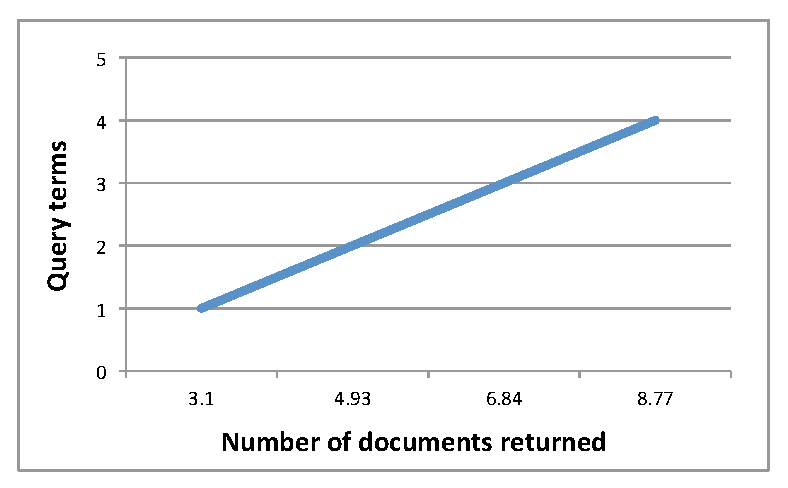
\includegraphics[width=4in]{queryterms-returnA.eps}
    \caption{ Length of the query and average returned documents for system A. }
    \label{Query structure}
\end{figure}

\begin{figure}[H]
    \centering
    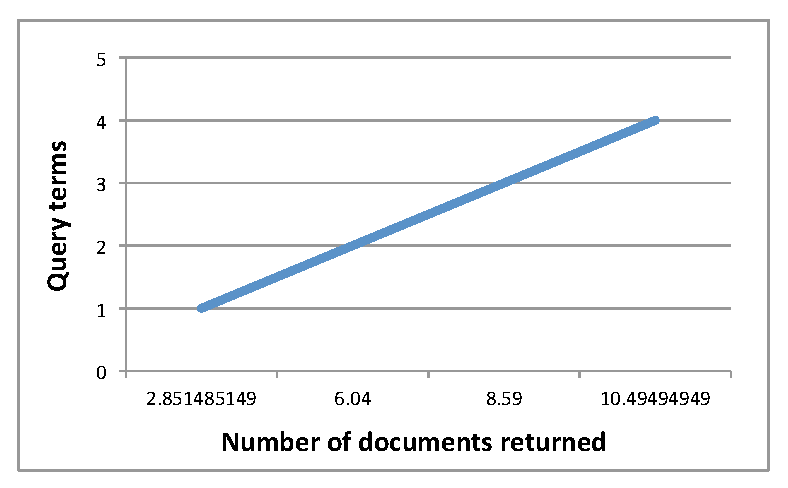
\includegraphics[width=4in]{queryterms-returnB.eps}
    \caption{ Length of the query and average returned documents for system B. }
    \label{Query structure}
\end{figure}

\begin{table}[h]
\centering
\caption { {\bf System A: Times in ms for each number of terms in the query } }
\begin{tabular}{llll}
\# Query terms & Minimum & Average & Maximum \\
1              & 0       & 1.32    & 11      \\
2              & 0       & 1.68    & 10      \\
3              & 0       & 2.38    & 17      \\
4              & 0       & 2.95    & 17       
\end{tabular}
\end{table}


\begin{table}[h]
\centering
\caption { {\bf System A: Number of returned documents each number of terms in the query } }
\begin{tabular}{llll}
\# Query terms & Minimum & Average & Maximum \\
1              & 1       & 3.01    & 20      \\
2              & 1       & 4.93    & 21      \\
3              & 1       & 6.84    & 30      \\
4              & 2       & 8.77    & 30       
\end{tabular}
\end{table}


\begin{table}[h]
\centering
\caption { {\bf System B: Times in ms for each number of terms in the query } }
\begin{tabular}{llll}
\# Query terms & Minimum & Average & Maximum \\
1              & 0       & 1.32    & 22      \\
2              & 0       & 1.21    & 14      \\
3              & 0       & 1.39    & 6      \\
4              & 0       & 1.60    & 11       
\end{tabular}
\end{table}

\begin{table}[h]
\centering
\caption { {\bf System B: Number of returned documents each number of terms in the query } }
\begin{tabular}{llll}
\# Query terms & Minimum & Average & Maximum \\
1              & 1       & 2.85    & 23      \\
2              & 1       & 6.04    & 24      \\
3              & 2       & 8.59    & 36      \\
4              & 2       & 10.49   & 36       
\end{tabular}
\end{table}


\subsection{ Accuracy }
We do our accuracy tests by implementing the following scheme. 
\begin{enumerate}
\item We choose randomly 20 words from the vocabulary database.
\item For each of these words we run the UWN database and we take, randomly,
four related words and we store it to a temporary structure. 
\item Using all of the above words we start creating documents, we create 
ten documents with 20 words inside each document.
\item The words to be put at each document are chosen in this way. In the 
first step, we choose 7 to 10 words from the vocabulary database. After this,
for each words from the chosen above we add 0 to 3 synonyms etc inside the 
documents.
\item We read the documents manually, we the humans, and then we created 
four queries with some relation to the words we read.
\item We input the queries to the system and we observe and evaluate the
results.
\end{enumerate}

Our findings are the following. The system in Phase A is worse in every aspect
such as Precision, Recall and F-measure and R-Precision. Still, it shows that 
the fallout is better from the system at Phase B. This is due to the fact that
we use extensively the UWN database to enrich the user's seach query. The 
weight we assign to the results of the UWN DB are static numbers and we reach 
to the conclusion that should be adjusted, even with feedback from the user, 
to provide more accurate results. Another point to bring up is that in order to
evaluate the system we need a more extended description on how to evaluate a
system and a proper common document collection to perform the evaluation with
predefined correct answers and their defined progression as returning results.


\section{Build instructions}
Our system was deployed with: {\tt Netbeans 8.0} and {\tt Java 1.7.0\_45}.Building instructions should be similar to other versions of Netbeans.

The following steps show to import the source and dependencies into a Netbeans project and build it from there.

\begin{enumerate}
	\item We create a new Netbeans Java project by \\
				{\tt File > New Project\ldots  > Java Project with Existing Sources }
	\item We name the project \emph{ Common} and the store location and press
				{\tt Next}
	\item We add the source folder located at the \emph{ Common} folder
				using {\tt Add folder\ldots}
	\item After the project is created, we import the \emph{ Stemmer} library
				located at {\tt Common\\dependencies}.
	\item We follow the steps 1 to 3 to create another project under the name "PonyIndexer" and we import the existing source files from the directory {\tt PonyIndexer\\src}.
	\item We again import the Stemmer library and this time we also import our created project "Common" by right-click on {\tt Libraries} of the "PonyIndexer" project and by following the steps of choice {\tt Add Project...}
	\item Final step is to build the project. Almost every package has it's own main and we can build the GUI separately.
\end{enumerate}

\section{Run instructions}
\begin{itemize}
	\item If you use Netbeans just Build \& Run.
	\item For a command line environment we simply change directory to {\tt \\dist} and we run the command {\tt java -jar NameOfJar.jar}. Please be make sure to copy all the necessary libraries.
	\item For the GUI, simply double-click the jar file.
\end{itemize}

\end{document}
